\section{Resultados}
Esta sección presenta la evaluación cuantitativa y cualitativa de las arquitecturas entrenadas.

\subsection{Evaluación Cuantitativa}
Los dos modelos fueron evaluados sobre el conjunto de validación independiente utilizando cuatro métricas de referencia: exactitud (Accuracy), puntuación F1 (F1-Score), área bajo la curva de características operativas del receptor (AUC-ROC) y el menor valor de la pérdida (Loss) en la convergencia.

\begin{figure}[htbp]
    \centering
    \begin{subfigure}[b]{0.48\textwidth}
        \centering
        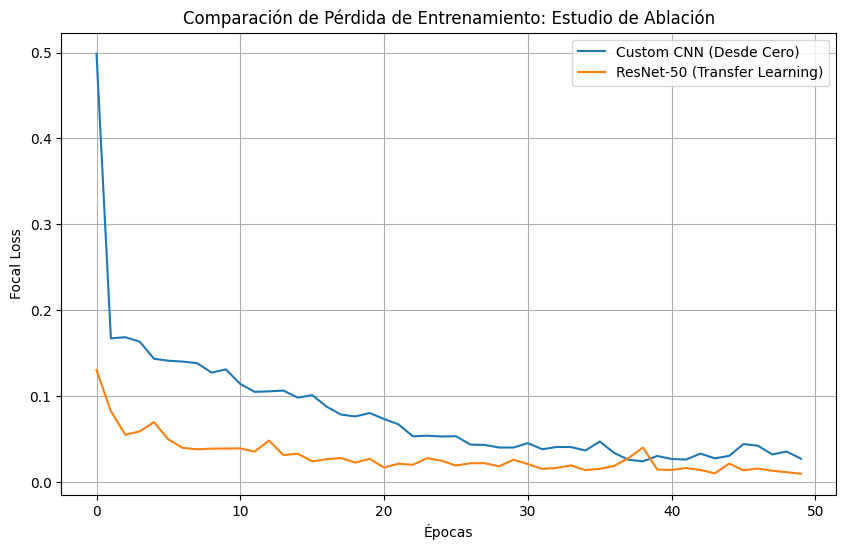
\includegraphics[width=\textwidth]{Imagenes/grafico_perdidas.png}
        \caption{Curvas de convergencia.}
        \label{fig:loss_sub}
    \end{subfigure}
    \hfill
    \begin{subfigure}[b]{0.48\textwidth}
        \centering
        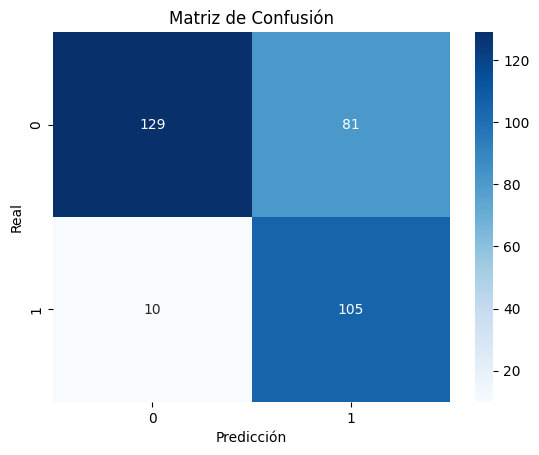
\includegraphics[width=\textwidth]{Imagenes/matriz_confusion.png}
        \caption{Matriz de confusión ResNet-50.}
        \label{fig:cm_sub}
    \end{subfigure}
    \caption{Comparación cuantitativa del entrenamiento y evaluación de los clasificadores de texturas.}
    \label{fig:evaluacion_cuantitativa}
\end{figure}

La Tabla~\ref{tab:resultados} resume el comportamiento comparativo del estudio de ablación.

\begin{table}[htbp]
  \caption{Métricas comparativas obtenidas en el estudio de ablación sobre el conjunto de validación.}
  \label{tab:resultados}
  \centering
  \begin{tabular}{lcccc}
    \toprule
    \textbf{Modelo} & \textbf{Exactitud (Accuracy)} & \textbf{F1-Score} & \textbf{AUC-ROC} & \textbf{Mejor Loss (Entr.)} \\
    \midrule
    Custom CNN (FL) & 66.77\% & 0.6400 & 0.7713 & 0.0244 \\
    ResNet-50 (FL) & 77.85\% & 0.7410 & \textbf{0.8928} & \textbf{0.0100} \\
    \textbf{ResNet-50 (BCE)} & \textbf{79.69\%} & \textbf{0.7537} & 0.8794 & 0.0725 \\
    \bottomrule
  \end{tabular}
\end{table}

Los resultados cuantitativos demuestran que el modelo \texttt{ResNet-50} supera ampliamente a la red \texttt{CustomCNN} en todas las métricas de clasificación. Específicamente, en la configuración con Focal Loss (FL), el AUC-ROC alcanza un valor de $0.8928$, lo que indica una alta capacidad de separación de clases de la red residual frente al $0.7713$ de la red convolucional básica. Además, la pérdida de entrenamiento se redujo considerablemente ($0.0100$ frente a $0.0244$). Por otro lado, la ablación de pérdidas muestra que el entrenamiento con \texttt{BCE} alcanza la mayor exactitud ($79.69\%$) y puntuación F1 ($0.7537$), aunque con un AUC-ROC levemente menor ($0.8794$) en comparación con \texttt{Focal Loss} ($0.8928$).

\subsection{Ajuste de Hiperparámetros (Learning Rate)}
En las pruebas rápidas de optimización de la tasa de aprendizaje para la ResNet-50 (con un tamaño de lote de 64, utilizando la regla de escalado lineal) se observó que:
\begin{itemize}
    \item Con una tasa de $2 \times 10^{-4}$ se obtuvo la convergencia más rápida y estable, consolidando una exactitud de validación rápida del 70.77\% en solo 5 épocas.
    \item Con una tasa de $1 \times 10^{-4}$ el aprendizaje fue estable pero más lento, logrando una exactitud inferior del 69.23\% en el mismo número de épocas evaluadas.
\end{itemize}

\subsection{Evaluación Cualitativa (Interpretabilidad)}
Para validar que la red de transferencia de aprendizaje toma sus decisiones basándose en características geométricas y texturales reales de los neumáticos y no en sesgos espaciales, se computaron los mapas de activación Grad-CAM sobre la última capa convolucional residual (\texttt{model\_resnet.layer4[-1]}).

\begin{figure}[htbp]
    \centering
    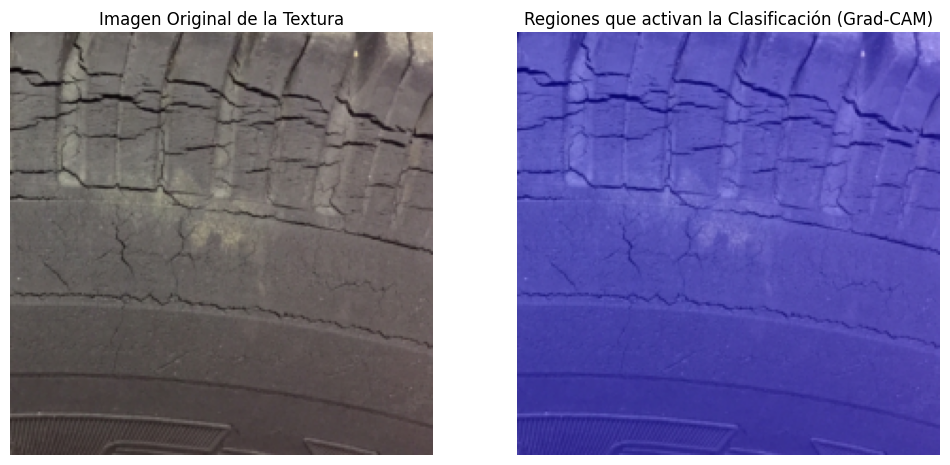
\includegraphics[width=0.7\textwidth]{Imagenes/gradcam_resultado.png}
    \caption{Visualización de activaciones mediante Grad-CAM sobre la textura del neumático, demostrando la concentración de atención en las grietas y zonas de desgaste.}
    \label{fig:gradcam}
\end{figure}

El examen cualitativo de la Figura~\ref{fig:gradcam} confirma que la red enfoca su atención de forma precisa sobre los surcos con grietas físicas o patrones lineales irregulares característicos de desgaste en la clase positiva (dañado), mientras que ignora el fondo homogéneo y el texto lateral de la llanta.
